\chapter{Source code version control}
\label{sec:source-code-version}

\section{Version control}
\label{sec:version-control}

What is version control? It is something as simple (and as difficult
to make right) as keeping track of changes in some piece of work, over
time. You
are probably familar with some very rudimentary version of version
control. Have you ever listed the documents in a folder and seen
something similar to this?

\begin{itemize}
\item myDocument
\item myDocument-2
\item myDocument-3
\item myDocument-final
\item myDocument-final2
\item myDocument-final-final
\item myDocument-definitive
\item myDocument-defitive-USE-THIS-ONE
\end{itemize}

If so, you already understand the most important idea behind version
control: our work is never created in one go, it changes over time and
sometimes we want to make sure we can go back in time to a former
version of it\ldots just in case. 

Many modern programs have version control embedded into them,
e.g. word processors like Microsoft Word, OpenOffice Write, or Google
Docs (also known as Google Drive). Very often they just track the
changes made to the document, sometimes they allow the user to go back
and forth in time to review, accept, or discard changes. This is also
very common in wiki sites like the Wikipedia. 

% TODO: add a screenshot of the version control in wikipedia here. 

Version control systems were initially created to track changes in
\emph{source code}. They were created by programmers for
programmers. We have come a long way since those days, and now version
control is spread over many different applications, but they still
pursue the same two goals: 

\begin{description}
\item[Reversibility: ] the capacity of going back in time if you mess
  up and introduce bugs in your code; sorry, \emph{when} you introduce
  bugs in your code.
\item[Concurrency: ] the capacity of working together with other
  people on the same project, on the same file, at the same time. 
\end{description}

These two capacities are basic for any modern programmer, and that is
why version control is (or should be) part of every programmer's daily
life. Modern programs are big and complex, and several programmers
work on them. Without appropriate version control, they cannot work at
the same time: they need to take turns, pass the baton\ldots this is
really unproductive, good programmers do not work like
that. Additionally, programmers ---even good programmers, as long as
they are human--- make mistakes all the time, sometimes serious
mistakes that break their programs completely, and they need to go
back in time to the point where everything was working fine and start
again (in large and complicated programs, this can be a long time
before).

In this chapter we will learn to make version control on your source
code files \emph{right}, not as shown above (e.g. myProgramOLD.groovy,
etc). We will use a program for doing so called \emph{Git}.

\section{Git}
\label{sec:git}

There are many programs for performing source code version control
nowadays. For this course, we are using Git, a version control system
created by Linus Torvalds, the same guy that created Linux. It is not
difficult to use but it is very powerful. 

Other very common version control systems are Subversion (also known
as svn) and Mercurial. There are many more. There are many sources
online, starting with Wikipedia, that will tell you the history of
version control, the differences between different systems, and much
more. I encourage you to go and read about it if you think the topic
is fascinating. If you just want to learn to use Git normally in
your life as a programmer, this section will help you learn the
basics. 

As you can imagine, a full book could be written about all the
possibilities and options that come with Git. Actually, several ones
have been published already. In this section I will just present the
most important 10\% of Git, which is all 
you will need 90\% of the time.  

\subsection{Starting a new project}
\label{sec:starting-new-project}

Let's start by creating a new programming project. Create a new folder
where you will put your programs. Now we want to start keeping track
of all changes. Assuming Git is installed in your system, and that you
are on the right folder, you only need to type \verb+git init+. With
this simple command, you have told Git to \emph{be ready} to keep 
track of whatever happens in this folder. So the full initialisation
of a complex complete version control system with Git looks like this: 

\begin{verbatim}
    > mkdir MyProject
    > cd MyProject
    > git init
\end{verbatim}

That was easy, wasn't it? Now you can keep track of all changes to
your files in this folder. Moving on\ldots

\subsection{Name and email address}
\label{sec:name-email-address}

Every time somebody makes a change to a program, Git marks the change
with the name and the email address of the person responsible for it. 
As you do not want to do is writing your
name and your email address every time you make a change, this is
usually set up at the beginning. You can do it with the command 
\verb+git config+. 

\begin{verbatim}
    > git config --global user.name "John Smith"
    > git config --global user.email "john.smith@student-bbk-ac-uk"
    > git config --global user.email "john.smith@gmail"
\end{verbatim}

These commands will set your name and email address for every (local)
repository in your machine because you are using the \verb+--global+
flag. 
%
A repository is just a place (somewhere in the internet) where the
source code for a project is stored. There are two types of 
repositories for any project:
local copies, where you do the work; and a public copy, that other
people can look at. 
Any machine on the internet can
be used to host a public copy of a Git project
and GitHub (\verb+www.github.com+) 
is a convenient place that
many people use. (We will use it too, but I will come to that later.)
%
Without the \verb+--global+ flag, 
the command modifies the configuration of
the current repository only. 
Sometimes you want to have different names or
emails on different repositories, although this is rare. 

Note that the email address does not need to be valid. To avoid spam,
it is not uncommon for users to use email addresses that are perfectly
understandable for human beings but confusing for spambots
(e.g. removing the last \verb+.com+ or changing dots for dashes.).

As with any other git command, remember that \verb+git help+ is your
friend. There is also plenty of online documentation. 

\subsection{Keeping track of changes}
\label{sec:keep-track-chang}

Now it is time to write some code. For example, we could create a
simple \emph{Hello World} application in Groovy. In other words, we
will edit a file called \verb+helloworld.groovy+ and write on it:

\begin{verbatim}
    print "Hello World!"
\end{verbatim}

If we execute this little program, it will print the words ``Hello
World!'' on the screen. So far, so good. Time to start filling up our
version journal! 

The first step is to tell Git that we want to keep track of this
file. In other words, we \emph{add} it to the list of files under
Git's responsibility. 

\begin{verbatim}
    > git add helloworld.groovy
\end{verbatim}

And now we must perform the most important operation in any version control
system: \emph{committing} our changes. 

\begin{verbatim}
    > git commit
\end{verbatim}

You will be asked to introduce some description of what this \emph{commit}
is about. Git automatically adds information about which files are
committed and what changes have been performed on them. The programmer
must provide some additional information: a short message to explain
to other programmers what the changes are about. Note that ``other
programmers'' can be yourself in two weeks time, when you have
forgotten what you committed at this point. Typical messages are
``First commit'', ``Fixed bug \#1304'', ``Added a new feature
for\ldots''; examples of bad non-informative commit messages are ``new
commit'', ``More code'', or ``Fixed it AT LAST!''. Write whatever you
want, but make a (small) effort to think what message will be useful
for people reading it in the future.

When you finish writing your commit description, save it and close the
editor. The commit will be performed, and you will be given some
output from Git. That output will include information about the
branch (by default, it is called \emph{master}), the identifier for
this commit (a unique identifier), your commit text, and some 
statistics about what the commit did: lines added, edited, or removed,
files added or removed, etc (\emph{see
  Figure~\ref{fig:git-example-1}}). 

\begin{figure}[htbp!]
  \centering
  \begin{framed}
    \begin{verbatim}
   > git commit
   [master 12a0006] Added the first line: just says "Hello World!"
   1 file changed, 7 insertions(+), 1 deletion(-)
   >
   \end{verbatim}
  \end{framed}
  \caption{Example of Git's output after a commit.}
  \label{fig:git-example-1}
  % TODO: add hand-written tags to screenshot
\end{figure}

Now your project has a history! It looks more or less like Figure~\ref{fig:git-example-2}.

\begin{figure}[htbp!]
  \centering
  
\includegraphics{gfx/no_figure.eps}
  \caption{Initial history of this project}
  \label{fig:git-example-2}
\end{figure}

Let's say we are not happy with our program. It does not do much. We
can modify the program to look like this:

\begin{verbatim}
    println "Hello World!"
    println "What's your name?"
    String s = System.console().readline()
    println "Hello " + s + "!"
\end{verbatim}

Now we can commit again (\verb+git add helloworld.groovy+;
\verb+git commit+, plus a commit description). Then we try to run
it\ldots Groovy will complain. We have messed up! At this point, we
have two options:

\begin{itemize}
\item If we know where the problem is (and in this simple example, we
  do) we can just fix it and commit again. A good commit message would
  be ``Fixed typo in line 3: readline() should be readLine()''.
\item If we did not know where the problem is, as it is usually the
  case in big programs, we can go back in time
  until we find the commit in
  which the problem started. Looking at the changes on that commit we
  can see how the \emph{bug} was introduced. Thanks to version
  control, finding bugs is much easier (and that is 80\% of the job). 
\end{itemize}

The simplest way to travel in time is by looking at the change log of
a file, and we are going to see how to do that in the next section. 

\subsection{Looking into the past}
\label{sec:looking-into-past}

Contrary to most novelists, programmers do not start working on a
project from a blank editor page. The most common situation is to work
on a project that has already been going on for some time. Maybe the
programmer is a new employee in the company, or has been transferred
to a different project, or has ``inherited'' a project that somebody
else started. It may be that the programmer wants to contribute to
another project because the project is appealing or
famous\footnote{Examples of interesting free/open-source projects with
  many contributors include web browsers like Firefox or Chrome, the
  Linux kernel, the Android operating system (based on Linux), the
  LibreOffice suite of applications, mail programs 
  like Thunderbird, and many others.}. Or maybe the programmer starts a
project from scratch and then realises that somebody else is doing the
same thing, only they started long ago and have made a lot of
progress, so it makes sense to join their team instead of reinventing
the wheel. For any of these reasons ---and many others--- you will
find yourself in a situation where you want to get a copy of the
source code that other people have written. This is very easy to do in
Git. You just need to be given a URL\footnote{A Uniform
  Resource Locator (URL) is a specific character string that
  constitutes a reference to an Internet resource. Examples of URLs
  are \texttt{http://www.bbk.ac.uk} and
  \texttt{ftp://gb.archive.ubuntu.com/ubuntu/}.
} to the source code, as
in the following example:

\begin{verbatim}
    > git clone https://github.com/bbk-msccs/currency-exchanger.git
\end{verbatim}

This is called \emph{cloning} the repository, for obvious reasons. 

Now that we have a copy of the Currency Exchanger project, let's look
at it. You will see that it has only two files: a ``read me'' file
called \verb+README.md+ (that explains what the project is about) and
a Groovy file called \verb+currencyConverter.groovy+. This is the
interesting one. 

Look at the code of \verb+currencyConverter.groovy+ and understand
what it does and how it works. Then come back and continue reading. Go
on, I will wait for you here. 

As you can imagine, this little program was not written in one go. You
can see a summary of the history of the file by looking at its
\emph{commit log}: 

\begin{verbatim}
    > git log currencyConverter.groovy
\end{verbatim}

This will show the list of commits on your screen, ordered
chronologically. For every commit, you can see the commit ID, the
author, and the date and time on which the commit was made. You can
also read the commit message. 

You can pass arguments to \verb+git log+ so that Git only shows you
commits for one author, or between two specific dates, and many
other options. Type \verb+git help log+ for more information. You can
use \verb+git help <command>+ to get help on any other command. 

The problem with \verb+git log+ is that it does not show how the code
changed from one commit to the next. But there is a way to do this:
\verb+git diff+. Let's have a look at an example: 

\begin{verbatim}
    > git diff ab9d6 9ecf9
\end{verbatim}

This command shows the changes between those two commits. Note that I
did not have to write the whole commit ID (40 characters!) but only
the first five are fine \emph{as long as they are unique}. If the
shortened IDs you use are not unique, Git will complain. In this case,
the short IDs are unique and Git tells that only one line was changed: 

\begin{verbatim}
    index 2d97cf4..5650842 100644
    --- a/currencyConverter.groovy
    +++ b/currencyConverter.groovy
    @@ -23,7 +23,7 @@ while (!finished) {
        case 2: 
            print "How many euro would you like to convert? ";
            double euro   = Double.parseDouble(System.console().readLine());
    -       double pounds = euro * poundOverEuroRatio;
    +       double pounds = pounds * euroOverPoundRatio;
            println euro + "€ will give you £" + pounds;
            break;
         case 0:  
\end{verbatim}

The ``-'' sign on the margin shows a deleted line while the ``+'' sign
shows an added line; the other lines were not changed. 
If you take everything into account, the only thing that changed
in this commit was the name of two variables on that line. 

\subsection{Sharing is caring}
\label{sec:sharing-caring}

\subsubsection{Push}
\label{sec:push}

If you wanted to improve this program, you could edit it yourself, add
new features, change some code, etc. You would commit regularly to
make sure you always have the history of your project up to date, so
you can see what changes you introduced over time. 

At some point you will want to make your changes public (in Git
jargon, this is called \emph{pushing your changes}), e.g. to allow
other members of your team to see what you have done. To make your
changes public, you usually need a place to put your \emph{public
repository} (as opposed to your \emph{local copy}, where you
work). You can host your public repository anywhere you want, but
GitHub is a convenient, well-known, and costless possibility. For the
purposes of this discussion, I will assume that you have an account at
GitHub, that your account name is ``ilovegit'', and that you have
created a repository in GitHub called ``my-currency-exchange''. 

The first thing you have to do (but you only need to do this the first
time) is telling Git where to push the changes. This is done by adding
a remote site (with the command\ldots \verb+git remote+, surprise!):

\begin{verbatim}
    > git remote add origin https://github.com/sergutsan/groovyck.git
\end{verbatim}

There are many things on that line that need explaining. First,
``add'' tells git that you want to add a new remote site; you can also
remove (``rm'') and rename (``rename'') remote sites. By default,
\verb+git remote+ will just show a list of your remote sites (name,
url\ldots). The word ``origin'' is just a name for the new remote site
to be used locally; origin is a common name for the main repository
where you push your changes. We could have used ``my-projects'', or
``myRemoteSite'', or any other name as long as we have not used it
yet. Finally, the URL is where the remote site
is. GitHub\footnote{GitHub does give you much more than just hosting
  your repositories: issue tracker, statistics, graphs, and limited
  social networking capabilities are some of the features you can use
  easily from their webpage. Not bad for a free service. Another good
  option is Google Code.} will give
you a URL that you can copy and paste (see Figure~\ref{fig:github}).

\begin{figure}[htbp]
  \centering
  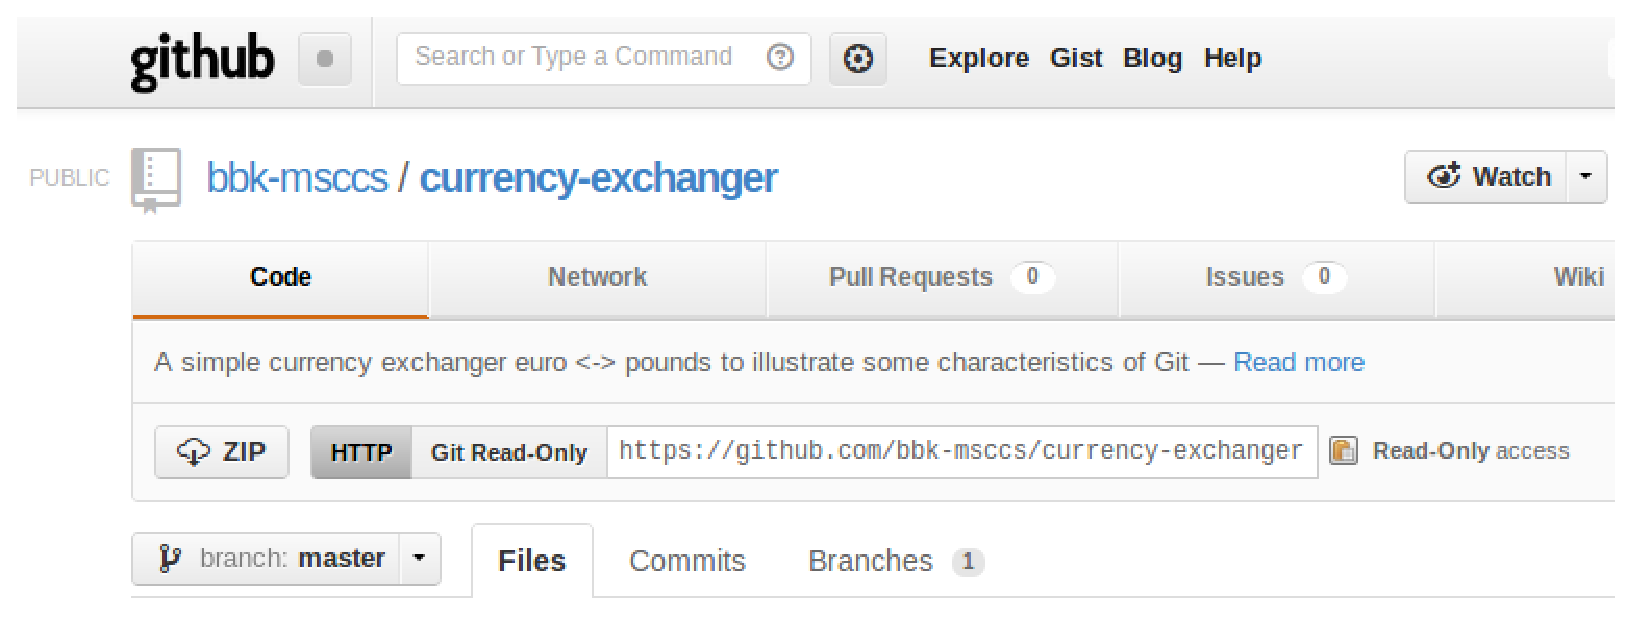
\includegraphics[width=\textwidth]{gfx/gitHubScreenshot.eps}
  \caption{Screenshot of GitHub. You can see the name of the user
    (``bbk-msccs''), the name of the repository
    (``currency-exchanger''), and the URL. You can use the URL both to
    clone the reposity and to push your changes (as long as this
    repository is yours, i.e. you can \emph{write} on it).}
  \label{fig:github}
\end{figure}

Once you have configured your remote repository or repositories,
pushing your changes is very easy: you only need to say where to push. 

\begin{verbatim}
    > git push origin 
    Username for 'https://github.com': ilovegit
    Password for 'https://ilovegit@github.com':
    To https://github.com/ilovegit/my-currency-exchange.git
    6457568..55ca3da  master -> master
\end{verbatim}

The system will ask for your username (``ilovegit'' in this example)
and your password. Then, if everything goes according to plan, 
it will inform you that it has pushed your commits. Note that 
this step could
fail for several reasons, like your network connection going down. 

\subsubsection{Pull}
\label{sec:pull}

Once you have pushed your changes, how do other people see them? How
do they take the code you have \emph{pushed} into your remote
repository and put in their local copies of the source code? As you
can imagine, they \emph{pull} it. 

\begin{verbatim}
    > git pull origin master
\end{verbatim}

When you pull, you have to specify the remote repository you are
pulling from (``origin'' in this case) and the branch you are pulling
from. We will talk later about branches, but for now it suffices to
say that the default branch in most projects is called ``master'', and
sometimes it is the only one. If you are not sure which branch you are
pulling from, ``master'' is usually a good guess.

Once you pull, Git will download the changes made public at that
public repository and merge them with your local copy. At this point,
you have the latest copy of the project's source code, including those
changes that somebody else (maybe you) made in a different computer. 

At this point, you have surely noticed that Git can be used to
synchronise with other team members, each other pulling whatever
changes others have pushed so that everybody is up to date; but it can
also be used to keep up to date with yourself: you can work on
different computers (at home, at the office, on your laptop on a
plane) and you can push your changes and then pull them from the other
computers. There is no need to carry around USB sticks with folders
called ``currencyExchangev2'', ``currencyExchangev3'', or
``currencyExchangev4usethisnottheother''. Git will always have the
latest version as long as you do not forget to commit and push
timely. 

\subsection{When should I commit?}
\label{sec:when-should-i}

As a general rule: \emph{commit early, commit often}. It is generally
a good idea to make small commits so that it is easier to go through
the history of your code and understand every step if you have to. The
cost of 
committing is almost zero so you should not be afraid of having too
many commits. There is no such thing. 

Of course, this does not mean that you commit every single character
that you write. Committing every single line is also probably too
much, unless those lines are really special (e.g.~they fix a bug). 
\emph{Do not spend more time
writing commit messages than writing code}. That said, if you have not
committed for the last half and hour, either you have written a lot of
code and you should commit early (as in \emph{now}); or you are tired
or distracted, and not really programming, so maybe you should have a
break.

If you are not sure what you have changed since the last commit, 
you can use \verb+git diff+. Another ---less verbose--- possibility
is to use \verb+git status+. The latter will tell you
which files have changed since the last commit, without details of the
changes.

Additionally, you should \emph{push} your changes to your public
repository fairly often. Some people say \emph{push early, push
  often}, but it does not mean that you need to push after every
commit. Sometimes 
you cannot even push because you do not have a network connection,
although this is becoming more and more uncommon these days, where you
can connect to the internet from planes, submarines, and almost a
robot wandering around Mars\footnote{Actually, a robot in Mars cannot
  connect to the internet, at least not what we call ``the Internet'' in
  2012. Radio waves travel \emph{only} as fast as light-speed, and it
  takes them so long to reach the Earth that internet hosts would
  timeout before a connection can be stablished. You could connect to
  the Internet from the Moon ---your bandwitdh would be
  very poor compared to your home connection, though.}. 
As a rule of thumb, push every time you 
have finished a coding session (e.g. before turning off the computer
or standing up to grab some lunch), or as soon as possible after that.


\subsection{Ignoring files}
\label{sec:ignoring-files}

Sometimes you want git to ignore some files. You do not want to keep
them under version control but cannot delete them, and do not want to
have them appearing on the screen every time that you check the status
of the repository. This is a common occurrence for temporary files
like \verb+.o+ files in C/C++, \verb+.class+ files in Java,
\verb+.dvi+ files in \LaTeX, automatic backup files, etc.

The way to tell Git to ignore these files is by listing them in a file
called \verb+.gitignore+ at the root of the repository. This file can
contain name files, but can also include wildcards. The typical
content of a \verb+.gitignore+ file can look like this:

\begin{verbatim}
    *.o
    *.class
    *~
\end{verbatim}

You can add comments to a \verb+.gitignore+ file (with ``\#''), add
exception to wildcard rules (with ``!''), and many more useful
tricks. Remember, \verb+git help gitignore+ is a good place to start
looking for help. 

The file \verb+.gitignore+ can be added and committed to your
repository like any other file.


% ADD INFO ON BRANCHES
% branch
% checkout % example: make the same algorithm in two different ways
%          % example: add a new class "in progress", that appears only
%          % in one branch and not the other
% merge


%%% Local Variables:
%%% mode: latex
%%% TeX-master: "main"
%%% End:

